\subsection{Modeling and Overview of the Testbed Distribution System}
This section presents a top-level overview of the proposed controller hardware-in-the-loop (CHIL) testbed designed to test any generic control algorithm in a real-time distribution system environment using DNP3 as the standard communication protocol. Fig. \ref{fig:overall_testbed} presents the overall infrastructure of the proposed CHIL testbed for grid-connected DERs. The testbed presented consists of the combination of the following components:


\begin{figure*}
\centering
  \noindent\makebox[\textwidth]{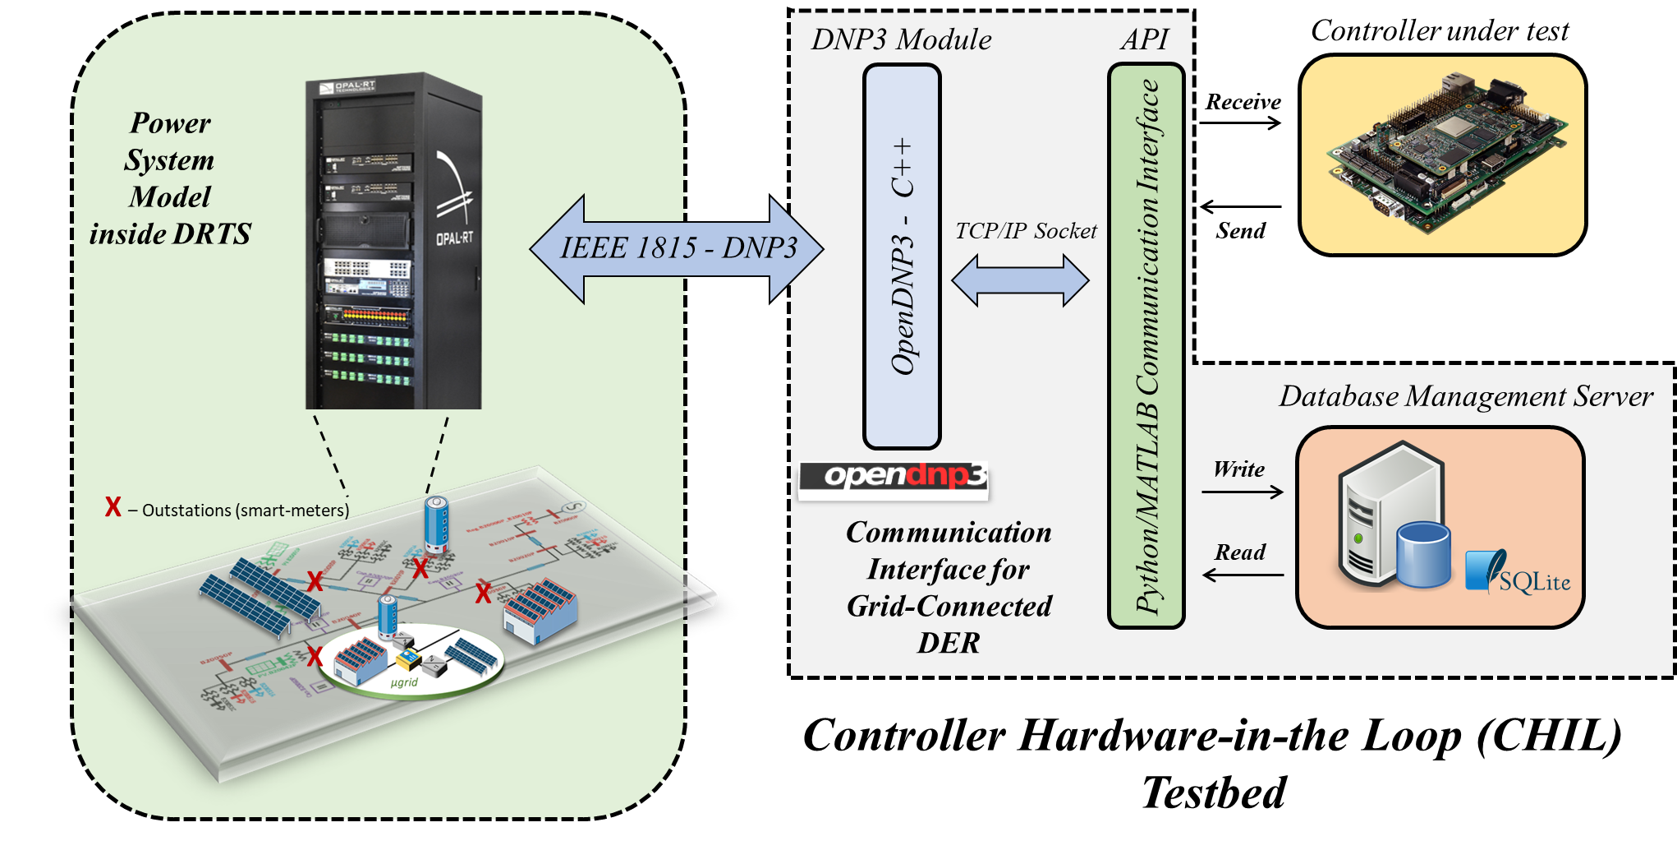
\includegraphics[width=14cm]{figs_juan/overall_testbed.png}}
  \caption{Top-level block diagram for the proposed controller hardware-in-the-loop testbed designed to test grid-connected distributed energy resources (DERs) in a real-time environment using IEEE 1815 DNP3 communication protocol.}
  \label{fig:overall_testbed}
\end{figure*}

\begin{itemize}
    \item \textbf{Real-time Distribution System Network Modeled Inside DRTS}: consists of different models designed to represent and simulate the behavior and interaction of grid-connected distributed energy resources (DERs) in a real-time environment. Some of these components are: a) Models for DERs (Lithium-ion batteries as energy storage systems (ES), Photovoltaic (PV) systems), b) Dynamic load models designed to simulate dynamic loading conditions,  c) Models for the distribution network, and d) Models for smart-meter devices designed to measure and communicate data such as voltages, currents, active power, and reactive power to the main (external) control system. All of these systems are modeled inside a digital real-time simulator (DRTS) with a 50-$\mu$s time step.
    
    
    \item \textbf{Communication Layer}: consists of a real-world-like communication infrastructure based on smart-meters models communicating with controllers using the IEEE 1815 DNP3 communication protocol. 
    
    
    \item \textbf{Controller-to-Simulation API Modules and Database Management Server}: consists of application programming interfaces (APIs) designed to provide inter-process communication to any generic control algorithm developed in MATLAB and/or Python. These API modules are designed to provide a communication bridge between the DNP3 communication module, a database management server, and any generic control algorithm devised to be deployed (and tested) in a real-time power system.
\end{itemize}



\subsection{Modeling of DER models and Dynamic Loading Conditions}
The modeling of all of the DER and load components that make up the power system model simulated inside the digital real-time simulator (DRTS) are described below.

\subsubsection{Photovoltaic (PV) System models}
The PV system model is based on a DC power source that simulates the PV array power output of the PV system given a power reference from real data obtained from large-scale solar PV plants located in the state of Florida. The PV system model also has a capacitor at the DC link, a three-phase pulse width modulated (PWM) voltage source converter (VSC), a LCL filter, and a transformer-based grid connection.


\subsubsection{Energy Storage Models}
The energy storage model used is based on a Li-Ion battery model available from MATLAB/SimPowerSystems. The charge and discharge behaviors of this battery model are presented in detail in  \cite{tremblay}. In general, this model was developed to provide predetermined behaviors for lead-acid, lithium-ion, nickel-cadmium and nickel-metal-hybrid batteries, and also simulate their temperature and aging effects. In addition to this model, a charge and discharge limiting function was developed to monitor the power control references requested by the algorithm under test while ensuring that the power demanded does not violate any system constraints.


\subsubsection{Dynamic Loads Models}
The load model used for the proposed system is based on a three-phase dynamic load profile in which the active (P) and the reactive power (Q) of the load changes dynamically based on predefined time criteria. The model used to represent the dynamic load connected to the distribution network is based on the dynamic load model available in Simscape Electrical\textsuperscript{TM} controlled using real load profiles obtained from measured nodes in an actual distribution network \cite{sungrin}. 

\subsubsection{Inverter Models for DER interconnection with the Distribution Network }An average-value based inverter model of a three-phase two-level voltage-source converter (VSC) is used as the central element for interconnecting DERs with the distribution feeder, dynamic loads, and other passive components. The DERs connected using the VSCs are the PV systems and the lithium-ion battery/energy storage (ES) systems. 

The independent control of the active and reactive power of the system is an essential capability needed for the power conditioning units (PCU) used to connect the DERs to the grid. That is why this is the selected technique for controlling the grid-connected DERs. This decoupled control of the powers allows the DERs to supply and absorb reactive power according to the needs of the system. For example, reactive power can be used to control voltages along the feeder. The control of the active power can be achieved by controlling the dc-link voltage, while the reactive power can be controlled by modifying the ac voltages at the converter terminals. By employing the \(abc-dq\) transformations and applying vector control, a \(dq\) decoupled control scheme can be developed to change the gating signals and change the power transfer dynamically without any interruption. The \(dq\) control scheme for VSC system is explained in detail in \cite{yazdani}. 




\subsection{Modeling of Distribution Network}
The modeling of the distribution network is performed using a reduced model approach, where reduced models of large distribution feeders are created to represent the behavior of the overall distribution network. In many cases, such as in our case, it is advantageous to reduce the level of detail of the model before performing the respective simulations due to the fact that this process can help us improve manageability and maintainability while improving the execution time and ability to run models in real-time. 

As an example of the advantage of using this reduced model approach, a reduced model for a large distribution feeder located in the state of Florida is used as the primary distribution system simulated inside the real-time simulator. This model was developed using field circuit information provided by utility companies. The main idea behind using the reduced model approach is that large portions of the system can be lumped into dynamic loads that can describe the behavior of a zone in the network. In essence, short laterals are lumped together while long laterals are kept in the model representation.

Fig. \ref{fig:modelreduction} shows an example of the sections used to convert the original distribution network model into a reduced feeder model \cite{sungrin}. It is important to mention that this reduced feeder model is the model used for the studies presented in this paper, but as seen, any distribution network topology can be used as the power system model simulated inside the DRTS.



\begin{figure}[!ht]
    \centering
    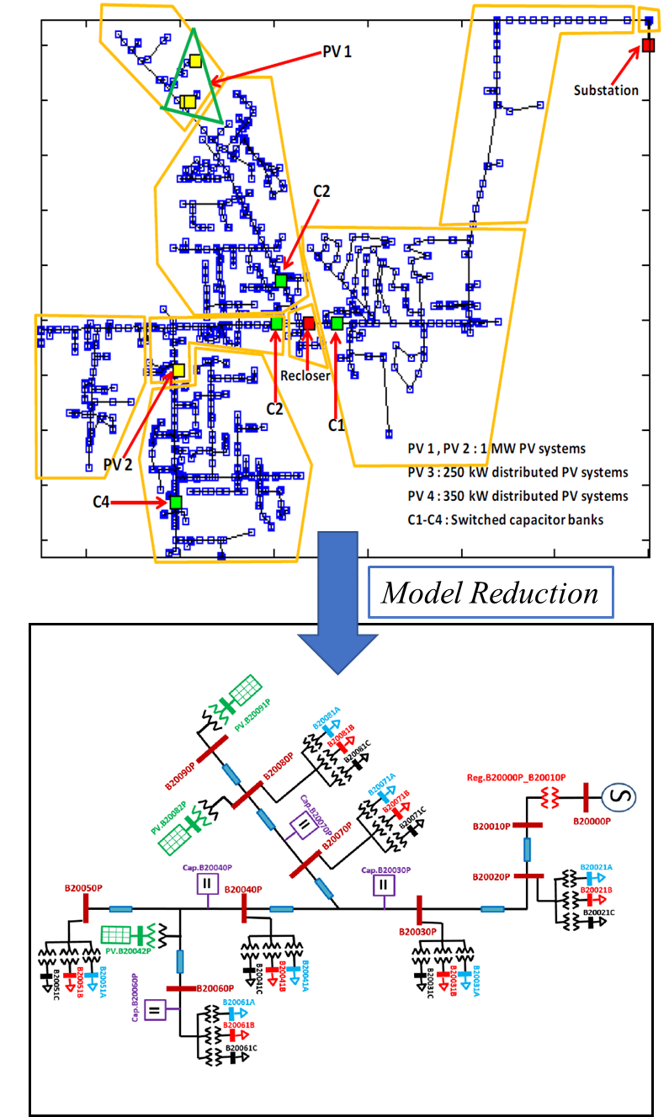
\includegraphics[width = 0.5\linewidth]{figs_juan/model_reduction.png}
    \caption{Model reduction approach applied to large distribution network. This model was reduced using circuit reduction and load aggregation.}
    \label{fig:modelreduction}
\end{figure}





\subsubsection{Modeling of Lines} The lines in the distribution network are modeled using $\pi$-model blocks. These lines are designed to simulate the behavior of distributed line sections based on the resistance, capacitance, and inductance specified on each line section. In essence, each line section of the distribution line was modeled as three $\pi$-model line sections in parallel, where the unbalanced conditions are preserved, and only the self-impedance of each line is taken into account. 


\subsection{Modeling of smart-meters inside the DRTS}
Models of smart-meter devices were developed to be deployed at different nodes in the distribution network in order to measure different states such as active power, reactive power, and single and three phase voltages and currents depending on the application. For example in an energy management application, the smart-meter models used can provide data such as the state-of-charge of multiple energy storage devices deployed at different nodes, current conditions of PV systems, and voltage measurements at critical buses.

Fig. \ref{fig:sm_meter} shows the block diagram of the smart-meter modeled inside the DRTS and deployed at different locations of the simulated power system. As seen in the picture, the frequency and voltage and/or currents of the node where the smart-meter is placed are the inputs into the smart-meter block. These inputs are then passed through an RMS conversion block and used to calculate other states of the system such as active and reactive power.

\begin{figure}[!ht]
    \centering
    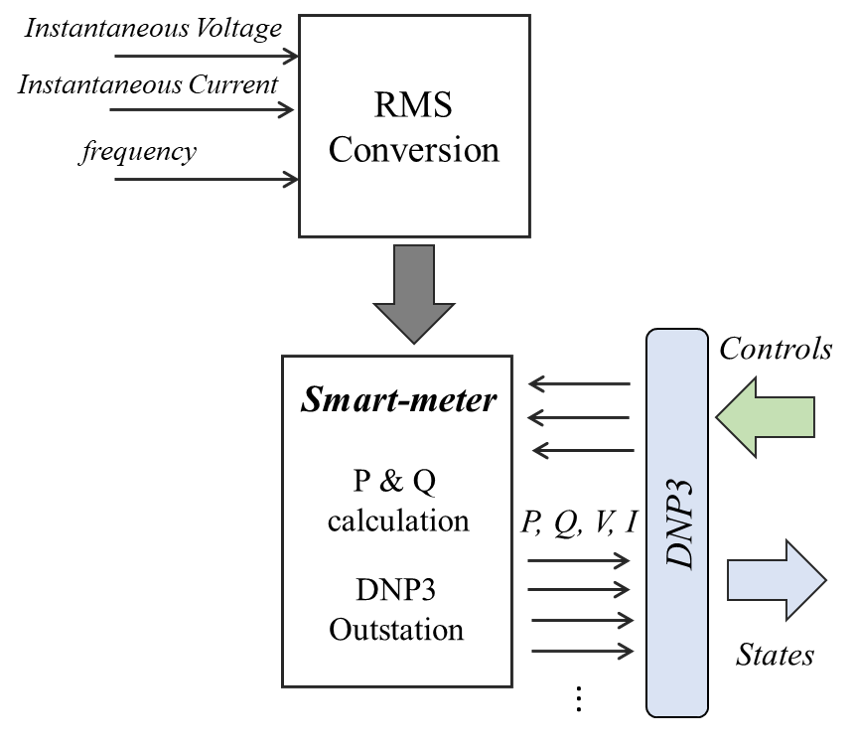
\includegraphics[width = 0.8\linewidth]{figs_juan/sm_meter.png}
    \caption{Block diagram for smart-meter modeled inside the digital real-time simulator (DRTS) communicating through DNP3 as outstations.}
    \label{fig:sm_meter}
\end{figure}



It is important to remember that all of these smart-meters were designed to communicate with external controllers, in a controller hardware-in-the-loop (CHIL) approach, using the DNP3 standard communication protocol. The APIs in charge of creating the "bridge" between any generic control algorithm (developed in MATLAB and/or Simulink) and the real-time power system simulation executing inside the DRTS are explained in detail in the next section. 


\subsection{Development of communication layer using DNP3 protocol and API modules.}
The chosen communication protocol used in the development of the communication layer of the testbed presented in this paper is the IEEE 1815 DNP3 protocol. This communication protocol provides several advantages when compared to other communication protocols when used for control applications deployed in distribution networks. One of these advantages is that DNP3 is an event-oriented protocol where devices are not required to be in constant communication thus significantly reducing the bandwidth requirements.

The DNP3 protocol is designed to determine the rules for the transmission of data from point $X$ to point $Y$ over serial or TCP/IP communication protocols. In the DNP3 protocol, a \textit{master} device is defined as the agent in charge of sending control commands and receiving the data coming from \textit{outstation} devices, in our case smart-meters, deployed at different locations of the system. These polling and posting procedures operate in two primary modes: a) \textbf{unsolicited response} and b) \textbf{event polling}. In the \textit{unsolicited response} mode of operation, the outstations only communicate data back to the master device if and only if the measurements have triggered a specific criterion. For example, when a voltage measurement goes out of bounds or when active and/or reactive power values fluctuate. This operating mode makes the DNP3 protocol ideal for applications where communication bandwidth is critical. Contrary, in the \textit{event polling} operating mode, the master controller needs to poll all the outstation devices individually looking for any changes in their data. If the data have not changed, then the response from the outstation will not contain any measurement data; otherwise, the new data will be transmitted from the outstation devices to the master.

As mentioned before, the DNP3 communication protocol is the primary communication protocol used for connecting the external controllers, or controllers under test (CUT), to the digital real-time simulation of the power system inside the DRTS. The right section of Fig. \ref{fig:overall_testbed} depicts how the information flows to and from the DRTS to the external controllers connected using a controller hardware-in-the-loop (CHIL) approach. It is important to observe in the figure that APIs were developed in both Python and MATLAB to serve as communication interfaces between any generic control algorithm, deployed in external controllers, and the DNP3 module in charge of communicating the data through DNP3 to the real-time model. These communication interface APIs are part of the contributions presented in this paper. A detailed explanation of the development of these communication interface APIs is given in the next section.